% *********************************************************************
% © 2010–2021 Jeremy Sylvestre
%
% Permission is granted to copy, distribute and/or modify this document
% under the terms of the GNU Free Documentation License, Version 1.3 or
% any later version published by the Free Software Foundation; with no
% Invariant Sections, no Front-Cover Texts, and no Back-Cover Texts. A
% copy of the license is included in the appendix entitled “GNU Free
% Documentation License” that appears in the output document of this
% PreTeXt source code. All trademarks™ are the registered® marks of
% their respective owners.
%
% *********************************************************************

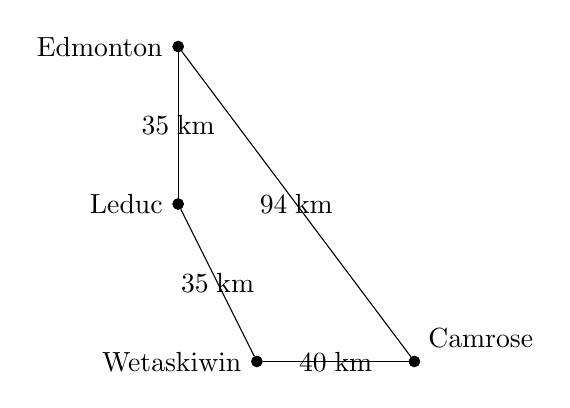
\begin{tikzpicture}[
	vertex/.style={ circle, draw, very thin, fill, inner sep=0pt, minimum size=4pt },
	vertexg/.style={ black!40!white, circle, draw, very thin, fill, inner sep=0pt, minimum size=4pt },
	vertexo/.style={ circle, draw, very thin, inner sep=0pt, minimum size=4pt }
]

\node at (-3,4) (e) [vertex,label=left:Edmonton] {};
\node at (0,0) (c) [vertex,label=above right:Camrose] {};
\draw (e) to node {$94 \; \mathrm{km}$} (c);
\node at (-2,0) (w) [vertex,label=left:Wetaskiwin] {};
\draw (c) to node {$40 \; \mathrm{km}$} (w);
\node at (-3,2) (l) [vertex,label=left:Leduc] {};
\draw (w) to node {$35 \; \mathrm{km}$} (l);
\draw (l) to node {$35 \; \mathrm{km}$} (e);

\end{tikzpicture}
